\subsection{Infinite Horizon LQR Formulierung}
    Der Ansatz beruht sich auf einen intuitiven Ansatz mit dem man beliebig einen trade-off zwischen Regelfehler und Regelfehler wählt. 
    
    LQR ist eine Abkürzung für \textit{linear quadratic regulator}. 
    \textbf{Linear:} da das System linear ist:
    \[\frac{d}{dt}x(t) = A\cdot x(t) + B\cdot u(t),\ x(t) \in \mathbb{R}^n,\ u(t) \in \mathbb{R}^m\]
    \textbf{Quadratic:} Definition einer  \textit{quadratischen} Kostenfunktion J:
    \[J(u(t)) = \int_0^\infty\Big(x(u(t))^T\cdot Q\cdot x(u(t)) + u(t)^T \cdot R \cdot u(t)\Big)dt\]
    der optimale Eingnang $u^*(t)$ minimiert die Kostenfunktion J:
     \[u^*(t) = \arg\min J(u(t))\]
     Die Zustände $x(t)$ und Eingänge $u(t)$ werden in Optimierungsproblem mit $Q$ und $R$ gewichtet, wobei 
     \[Q=Q^T \in \mathbb{R}^{n\times n},\ Q \succeq 0,\ \textnormal{und}\ R = R^T \in \mathbb{R}^{m\times m},\ R\succ 0\]
     Die Definitheit der Matrizen $Q$ und $R$ ist notwendig, damit das Argument des Integrals quadratisch konvex ist.
     Somit ist das Minimum von $J(u)$ einzigartig, falls es existiert.
    
    \textbf{Regulator:}
    der Reglerlösst das \textit{regulator} Problem:
    \[\lim\limits_{t \to \infty}x(t)=0\]
    
    % Das heisst der Regler bringt den Zustandsvektor in unendlicher Zeit in seinen Ursprung.
    
    % \textbf{Zusammenfassend:}
    % LQR-Formulierung
    % \[\min J(u),\]
    % unter der Berücksichtigung der Dynamik:
    % \[\frac{d}{dt}x(t) =A\cdot x(t) + \cdot u(t),\]
    % wobei $Q$ und $R$ einstellbare Grössen sind. 
    % Beispielhaft werden zwei Fälle betrachtet:
    
    $\boxed{Q\uparrow \widehat{=}\, R \downarrow}$ je grösser $Q$ relativ zu $R$, desto teurer ist es wenn $x(t)$ nicht im Ursprung ist. Das System wird schnell an den Ursprung geregelt, um die Kosten tiefstmöglich zu halten. Dabei wird $u(t)$ jedoch betragsmässig gross sein.
    
    $\boxed{Q\downarrow \widehat{=}\, R \uparrow}$ je grösser $R$ relativ zu $Q$, desto teurer ist es viel Energie mit den Ausgangsgrössen auszugeben. Das System wird langsam (mit betragsmässig kleinem Regelsignal $u(t)$) in den Ursprung geregelt.
    
    Note: eine Erhöhung der Eigenwerte von $Q$ hat den gleichen Effekt wie eine Reduzierung derer von $R$. Die relative Grösse ist von Relevanz.
    
    \subsubsection{Eigenschaften von Infinite Horizon Reglern}
    \textbf{Stabilität:}
        Die Matrix $A-B\cdot K$ des geschlossenen Regelkreises ist garantiert Hurwitz (stabil).
        \begin{equation*}
            \colorboxed{red}{\Dot{x}(t) = \big(A - B\cdot K\big) \cdot x(t)}
        \end{equation*}
    
    \textbf{Robustheit:}
        Für die Wahl $R=r\cdot I$ hat die minimum return difference $\mu_{min}$ folgende Eigenschaft:\[\mu_{min,LQR} = \min_{\omega}\Big(\min_{i}\ \sigma_i(I+L_{LQR}(j\omega))\Big) \geq 1 \]
        
        Im SISO-Fall lässt sich diese Eigenschaft folgendermassen darstellen.
        Dies garantiert eine Verstärkungsreserve von $\gamma \in [\,0.5, \infty)$ und eine Phasenreserve von $\varphi \geq 60^\circ$
        
    \begin{figure}[H]
        \centering
        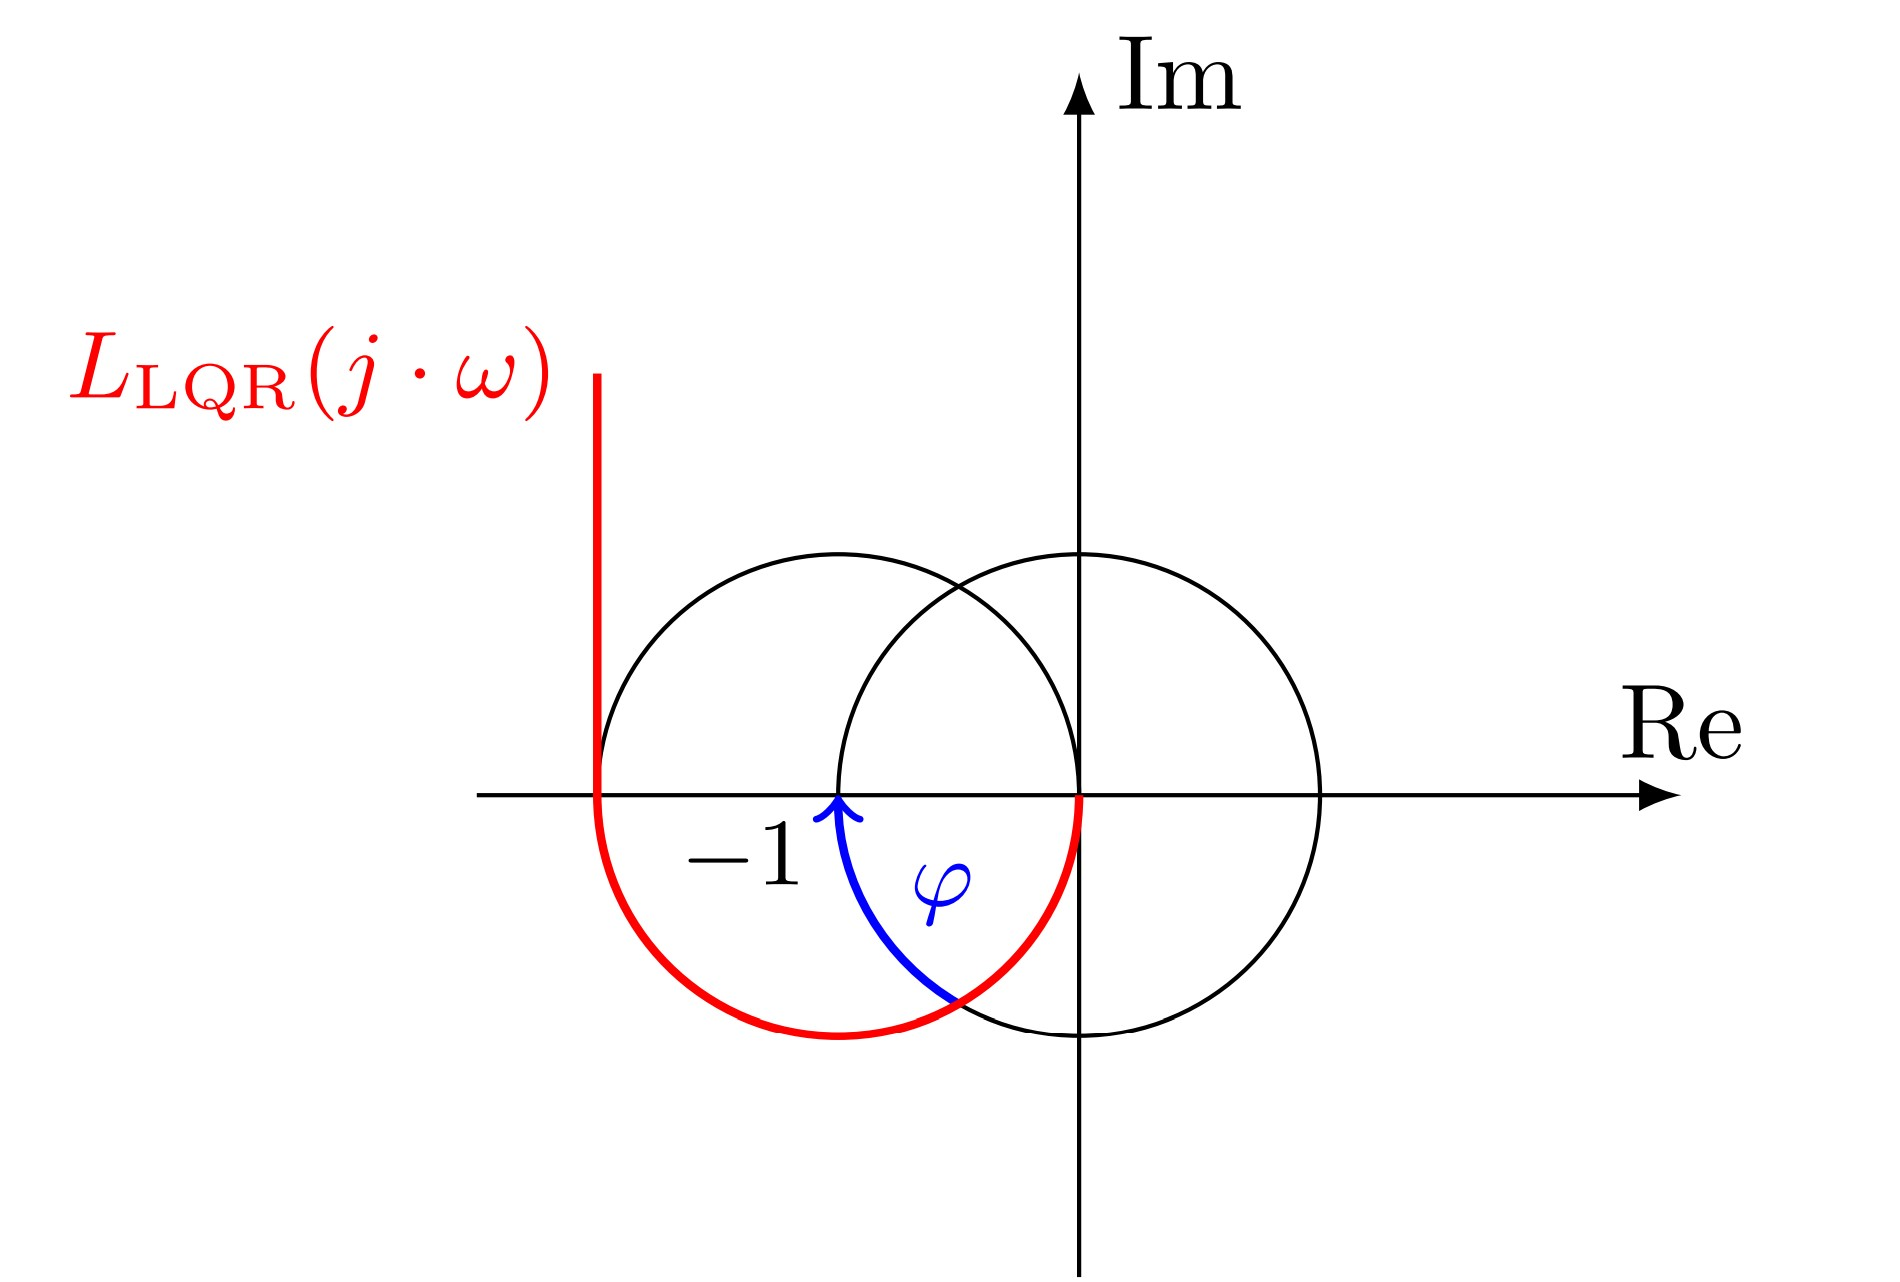
\includegraphics[width = 0.6 \linewidth]{images/08/SISO_Robustheit.jpg}
    \end{figure}
    
    Durch modifizieren der Riccati-Gleichung mit $\beta > 1$ wie folgt:
    \[\frac{1}{\beta}\cdot\Phi_\beta\cdot B\cdot R^{-1}\cdot B^T\cdot \Phi_\beta - \Phi_\beta \cdot A - A^T\cdot \Phi_\beta-Q = 0\]
    
    so resultiert die Lösung $\Phi_\beta$. Damit wird der Regelkreis noch robuster, da dann gilt: 
    
    \[\mu_{min,LQR}=\min_\omega\Big(\min_{i}\ \sigma_i(\beta I+L_{LQR}(j\omega))\Big) \geq \beta \]
    
    Das heisst, der Nyquist-Plot tritt nie in den um $-\beta +j\cdot0$ zentrierten Kreis mit Radius $\beta$ ein.
    
    